\chapter{Resultate}
\label{ch_resultat}

Im Kapitel \ref{ch_vorgehen} ist die Umsetzung ausführlich erklärt. In diesem Kapitel geht es um die relevanten Resultate. Beim Harvester geht es um den produzierten Print, die Leistungsfähigkeit der Schaltung, und die Qualität des Signals am Harvesterausgang. Beim Energy Management wird das Verhalten mit den finalen Schwellwerten dokumentiert. Einerseits geht es um die Kontrolle der eingestellten Schwellwerte sowie um die erreichte Ladezeit des Primärspeichers STS. Es wird zusammengefasst, bei welcher Geschwindigkeit wie oft BLE-Pakete gesendet werden. Das Verhalten wird im Unterkapitel durch die Energiebilanz gedeutet. Der Zusammenhang zwischen der Geschwindigkeit und dem realen Verbrauch des TI-Sensortags wird für ein erstes Anfahren und für das Weiterfahren beschrieben. Der Vorteil des Weiterfahrens ist, dass die Kondensatoren in diesem Fall bereits geladen sind. Als letztes wird das User Interface der neuen BLE-Applikation gezeigt.
 
\section{Harvesterschaltung}

Nachfolgend werden die Resultate, der Harvesterschaltung beschrieben. Die Energie, welche die Harvesterschaltung zur Verfügung stellt liegt im $\mu$J-Bereich, das nachfolgende Energymanagement muss mit dieser Energie arbeiten können.

\subsection{Der Print}

Die erstellte Leiterplatte ist in den Abbildungen \ref{print_rueckseite} und \ref{print_vorne} zu sehen. Auf der Ansicht von oben ist der Top-Layer inklusive der Bestückung zu sehen. Die Bestückung des Top-Layers beinhaltet die Harvesterschaltung (unten rechts), den EM8500 (oben rechts) und den Stecker (mittig links), welcher als Verbindung zum TI-SensorTag dient. Ebenfalls sind die vielen Testpunkte zu sehen. Jedes Netz wurde mit einem Testpunkt ausgestattet. Oben links sind die Anschlüsse für die Energiespeicher zu sehen. Hier wurden die beiden Elektrolytkondensatoren, kurz Elkos, über Litzen angeschlossen. Die Elkos können nicht auf der Oberseite der Leiterplatte platziert werden, da der Platz zwischen TI-SensorTag und dem Prototypen-PCB nicht ausreicht und auf der Unterseite ist kein Platz, da die Speiche des Fahrrads in einem Abstand von ein bis zwei Zentimeter vorbei schnellt. 

Auf der Ansicht von unten ist der Bottom-Layer inklusive der Bestückung zu sehen. Die Unterseite der Leiterplatte beherbergt die Spule und den Reed-Switch. Der Reed-Switch hätte noch Platz auf der oberen Seite gehabt, jedoch muss der Reed-Switch in der Nähe der Spule platziert werden, da hier der Magnet durchläuft.

\begin{figure}[ht]
 \begin{minipage}[t]{0.5\textwidth}
    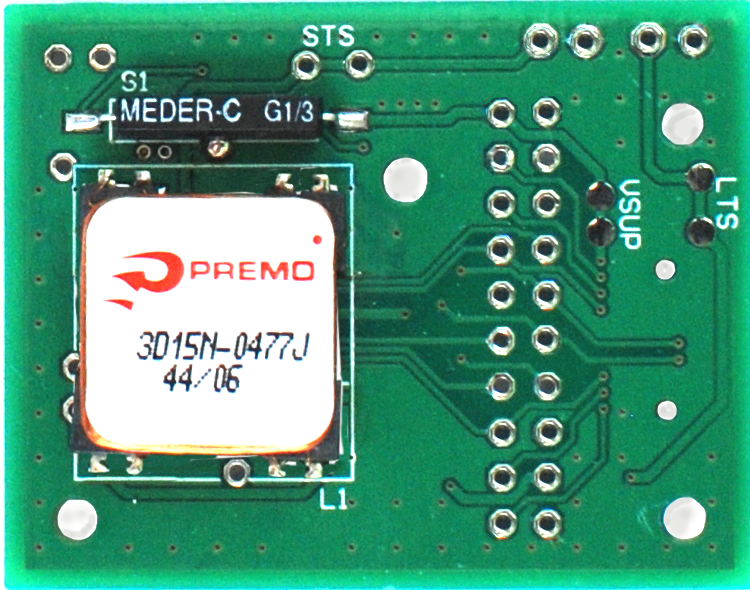
\includegraphics[width=0.9\textwidth]{4Resultate/imag/print_rueckseite.png} 
    \caption{Print Ansicht von unten}
    \label{print_rueckseite}
 \end{minipage}
 \begin{minipage}[t]{0.5\textwidth}
    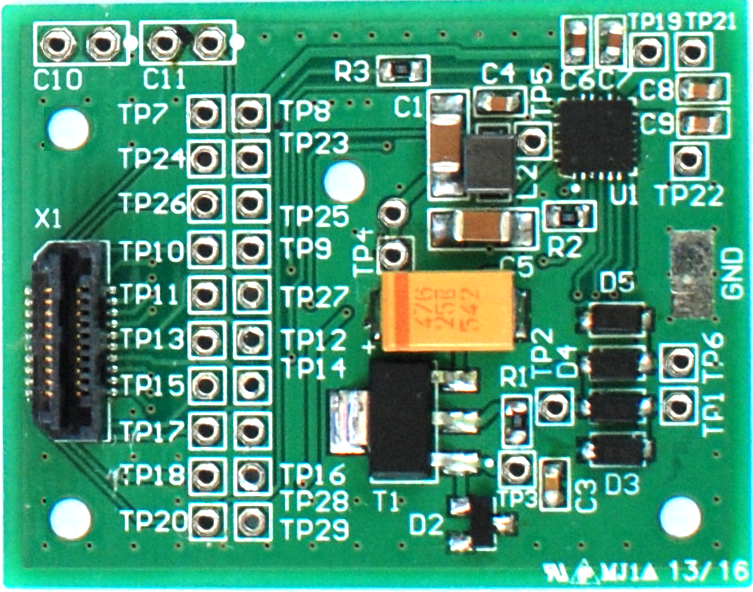
\includegraphics[width=0.9\textwidth]{4Resultate/imag/print_vorne.png} 
    \caption{Print Ansicht von oben}
    \label{print_vorne}
 \end{minipage}
\end{figure}

\subsection{Leistung am Harvesterausgang}

Wie erwartet (siehe theoretische Grundlagen Unterkapitel 2.1.3 Abschnitt \ref{mpp_theorie_diff}) ändert sich bei einer Hardware mit einer Spule das Leistungsmaximum. Die Abbildung \ref{mpp_resultat_harvester} zeigt die reale MPP-Kurve des Prototypen. Bei verschiedenen Geschwindigkeiten ist der MPP an einem anderen Punkt. Problematisch ist, dass die Einstellung im EM8500 nicht so genau eingestellt werden kann. Es sind nur grobe Schritte im Bereich von 50 - 70 \% verfügbar. 

\begin{figure}[ht]
    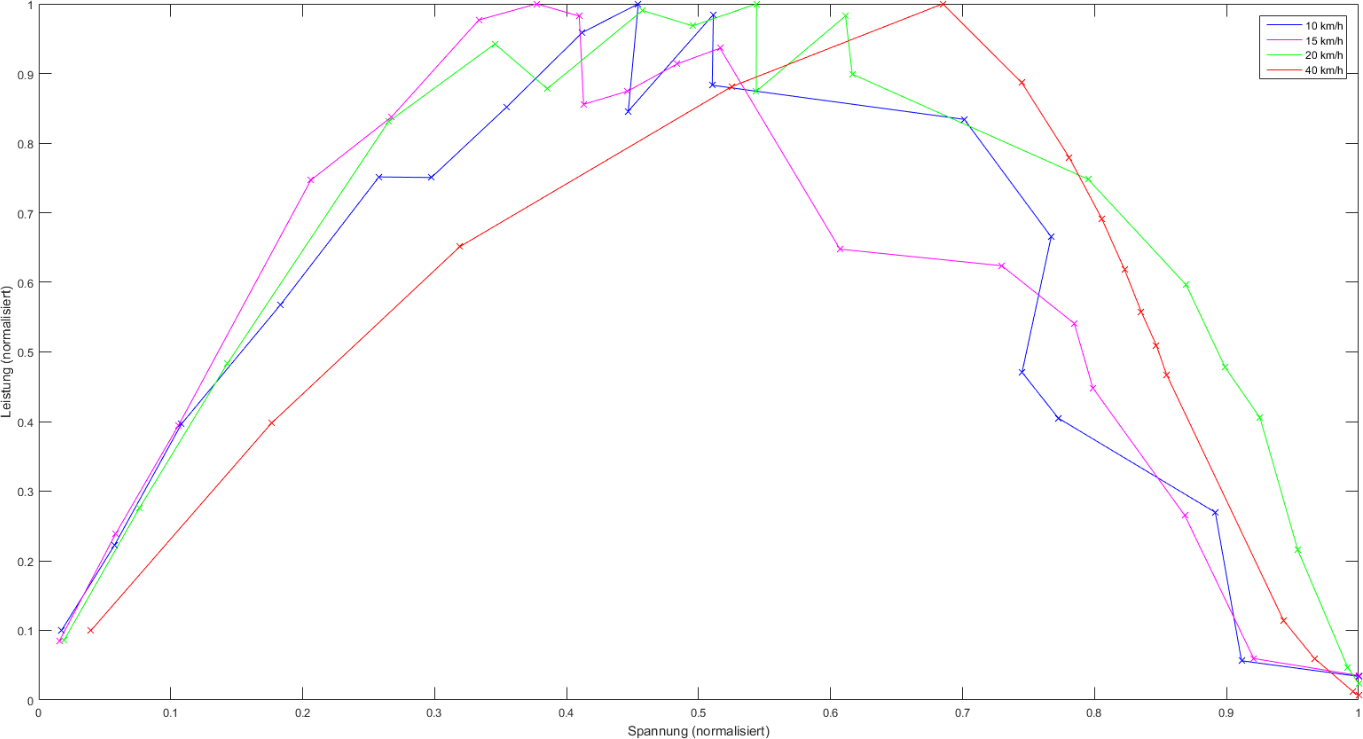
\includegraphics[width=0.5\textwidth]{4Resultate/imag/MPPHarvester.png} 
    \caption{Leistungskurve Harvesterausgang (normalisiert)}
    \label{mpp_resultat_harvester}
\end{figure}

Die Leistung, welche der Harvester zur Verfügung stellen kann, liegt bereits bei einer Geschwindigkeit von 10 km/h bei 24.77 $\mu$W. Dies ist die Durchschnittsleistung bei optimaler Belastung. Es handelt sich nicht um die Spitzenleistung. In der Tabelle \ref{leistungHarvester} ist es ersichtlich, dass die Leistung mit der steigender Geschwindigkeit zunimmt.

\begin{minipage}{\textwidth}
\captionof{table}{Leistung Harvesterschaltung Bicycle Computer}
    \label{leistungHarvester}
    \begin{tabbing}
        Geschwindigkeit \quad\= Leistung Harvester \\[0.8ex]
        10 km/h  \> 24.77  $\mu$W \\
        15 km/h  \> 61.07  $\mu$W \\
        20 km/h \> 116.69 $\mu$W \\
        40 km/h \> 472.61 $\mu$W \\
    \end{tabbing}
\end{minipage}

Es ist zu beachten, dass diese Werte die Leistung des MPP sind, somit können diese Leistungen nur erreicht werden, wenn die Einstellung des EM8500-Chips dementsprechend eingestellt werden.


\subsection{Verhalten des Harvesterausgangs}

Die Abbildung \ref{resultat_Harvester_Spannung_47uF} zeigt das Verhalten des Harvesterausgangs mit einem 47 $\mu$F Elko bei der Belastung durch den EM8500-Chip. Die Spannung ist über einen längeren Zeitraum betrachtet sehr instabil. Diese Problematik wurde bereits im Kapitel \ref{Ausmessen der Auswirkung des Ausgangskondensators} beschrieben. Die Abbildung \ref{resultat_Harvester_Spannung_100uF} zeigt das reelle Verhalten des Harvesterausgangs mit einem 100 $\mu$F Elko. Es ist zu sehen, dass die Spannung am Harvesterausgang über einen längeren Zeitraum relativ konstant bleibt. Genaue Messdaten zu dieser Problematik sind im Messprotokoll \cite{messung_harvester_elko} zu finden.

\begin{figure}[ht]
 \begin{minipage}[t]{0.5\textwidth}
    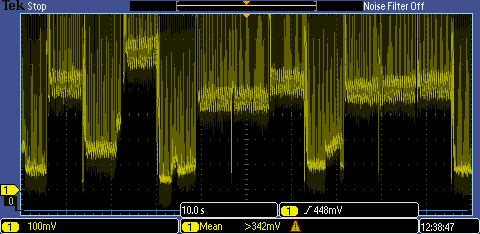
\includegraphics[width=0.9\textwidth]{4Resultate/imag/SpannungVCC_47uF.PNG} 
    \caption{Spannung VCC beim Harvesterausgang mit 47 $\mu$F}
    \label{resultat_Harvester_Spannung_47uF}
 \end{minipage}
 \begin{minipage}[t]{0.5\textwidth}
    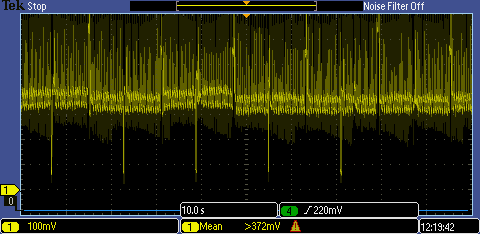
\includegraphics[width=0.9\textwidth]{4Resultate/imag/SpannungVCC_100uF.png} 
    \caption{Spannung VCC beim Harvesterausgang mit 100 $\mu$F}
    \label{resultat_Harvester_Spannung_100uF}
 \end{minipage}
\end{figure}

\subsection{Energie am EM8500-Chipausgang}

Die Abbildung \ref{energie_resultat_harvester} zeigt die berechnete Energie, die am Ausgang des EM-Chip abgegeben wird in Bezug zur Geschwindigkeit. Die Berechnung, wie aus dem Puls über die Zeit, bis dass VSUP wieder eingeschalten wird, ist im  Messprotokoll \cite{messung_emausgang_finish} dokumentiert. Die gewonnene Leistung, die dem TI-SensorTag zur Verfügung steht ist:


\begin{minipage}{\textwidth}
\captionof{table}{Leistung EM8500-Chip-Ausgang}
    \label{res_em_aus}
    \begin{tabbing}
        Geschwindigkeit \quad\= Leistung EM8500\_out \\[0.8ex]
        10 km/h  \> 5.44   $\mu$W\\
        15 km/h  \> 20.91  $\mu$W\\
        20 km/h  \> 41.39  $\mu$W\\
        40 km/h  \> 170.75 $\mu$W\\
    \end{tabbing}
\end{minipage}


\begin{figure}[ht]
    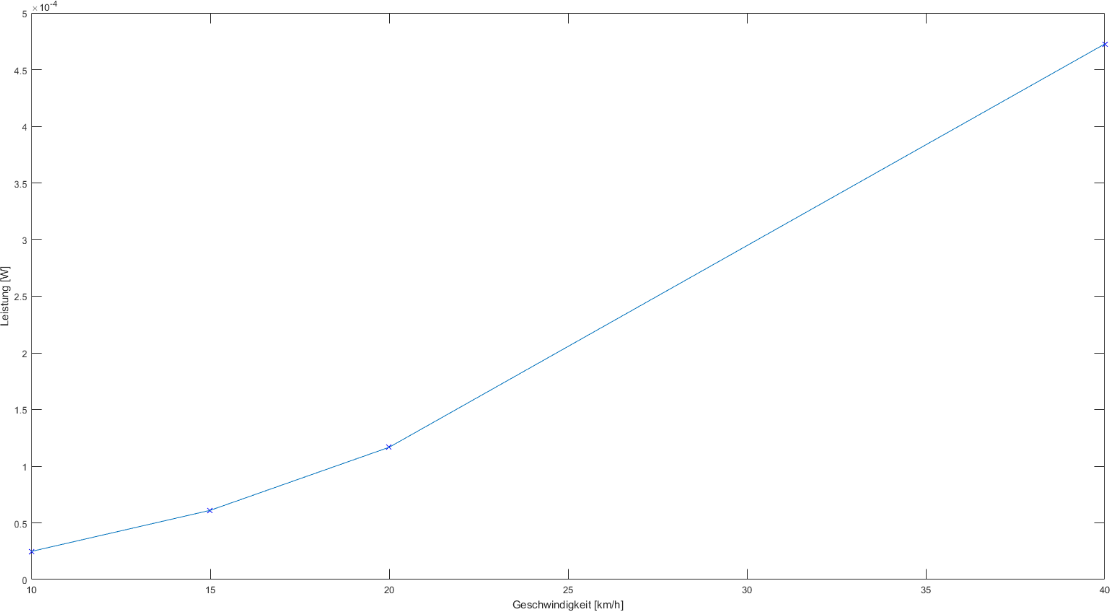
\includegraphics[width=0.5\textwidth]{4Resultate/imag/ResultatLeistungGeschwindigkeit.png} 
    \caption{Maximale Leistung vs. Geschwindigkeit}
    \label{energie_resultat_harvester}
\end{figure}

\subsection{Wirkungsgrad des Bicycle Computers}

Aus den zwei Leistungsmessungen wird graphisch die Energiegewinnung im Vergleich dargestellt (Abbildung \ref{zsmEnergyGewinn}). Die Werte beziehen sich auf die gemittelte Leistung über 10 s. Es ist zu sehen, dass die Energiegewinnung bei der Harvesterschaltung mit der Geschwindigkeit deutlich schneller zunimmt als die Energie am Ausgang des EM-Chips. 

\begin{figure}[ht]
    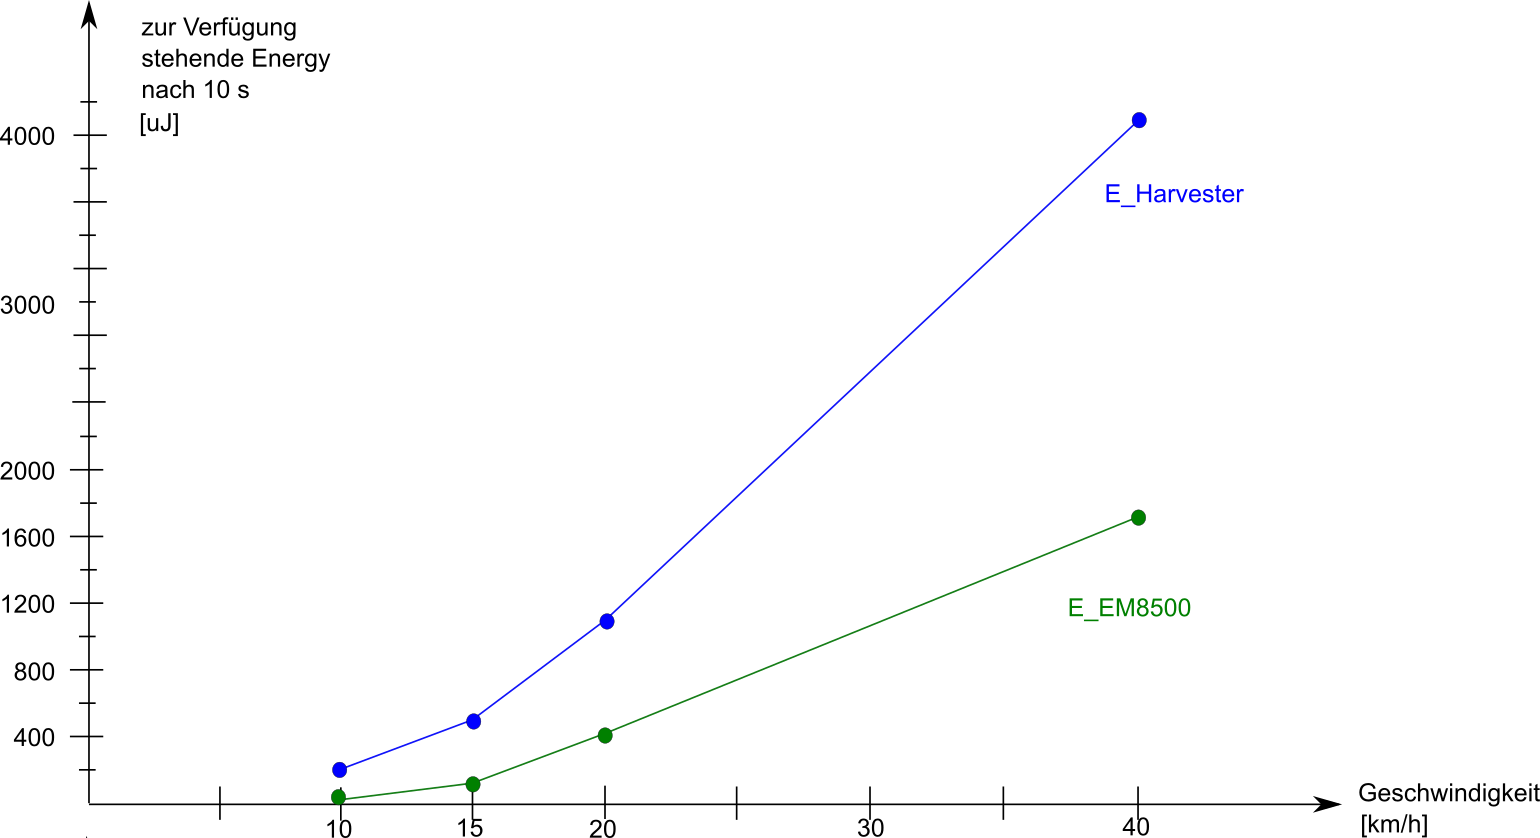
\includegraphics[width=1\textwidth]{4Resultate/imag/EnergyGewinnNachStelle.png} 
    \caption{Energiegewinn Zusammengefasst an zwei Messpunkten}
    \label{zsmEnergyGewinn}
\end{figure}

Aus den zwei Leistungsmessungen wurde der Wirkungsgrad bei den gemessenen Geschwindigkeiten berechnet (siehe Tabelle \ref{wirkungsgrad_emchip}). Der Wirkungsgrad ist bei tiefen Geschwindigkeiten sehr schlecht (24.87\thinspace\%). Dies ist eine der zwei Ursachen, dass trotz genug geernteter Energie das TI-SensorTag für das Senden der Sensorwerte bei tiefer Geschwindigkeiten nicht wie erwartet genug Energie hat. Mit mehr Geschwindigkeit erhöht sich nicht nur die geerntete Leistung rapide, sondern auch der Wirkungsgrad (siehe Tabelle \ref{wirkungsgrad_emchip}). Der Wirkungsgrad des EM8500 innerhalb des entwickelten Prototypen liegt bei 40 km/h  bei 41.01\thinspace\%.  

\begin{minipage}{\textwidth}
\captionof{table}{Wirkungsgrad Bicycle Computer nach Geschwindigkeiten}
    \label{wirkungsgrad_emchip}
    \begin{tabbing}
        Geschwindigkeit \quad\= Leistung Harvester \quad\= Leistung EM8500\_out \quad\= Wirkungsgrad\\[0.8ex]
        10 km/h  \> 21.87  $\mu$W \> 5.44   $\mu$W \> 24.87\thinspace\%  \\
        15 km/h  \> 57.19  $\mu$W \> 20.91  $\mu$W \> 36.56\thinspace\%  \\
        20 km/h \> 114.67 $\mu$W \> 41.39  $\mu$W \> 36.09\thinspace\%  \\
        40 km/h \> 416.29 $\mu$W \> 170.75 $\mu$W \> 41.01\thinspace\%  \\
    \end{tabbing}
\end{minipage}  


\section{Energy Management}

Im Kapitel Vorgehen ist die Einteilung der Energiezustände in LOW, MIDDLE und HIGH ENERGY beschrieben (\ref{v_energiezustand}). Die folgenden Abbildungen im Unterkapitel \ref{tiefes_v} zeigen diese Verhalten. Zuerst wird das Verhalten bei LOW und MIDDLE ENERGY beschrieben. Da interessiert die Ladezeit bis dass wieder ein Paket gesendet wird. Bei beiden Zuständen kann sich der LTS nicht laden, da das Senden über BLE alle Energie verbraucht. Erst bei höherer Energie kann das Ladeverhalten von LTS angeschaut werden. Diese Abbildungen sind im Unterkapitel \ref{res_entladen}. Im letzten Unterkapitel stehen die finalen Schwellwerte und Kondensatorenwerte, auf denen diese Messresultate basieren.

\subsection{Verhalten bei tiefen und mittleren Geschwindigkeiten}
\label{tiefes_v}


Das Primärziel, dass der Energy Harvesting Powered Bicycle Computer bei 10 km/h BLE-Pakete erhält ist gemäss Abbildung \ref{paket_100kmh} gelungen. Nach rund 40 Sekunden sendet der Fahrrad-Computer neue Daten. Das rote Signal ist die Speisung V\_SUP, die nach dem erreichen des Schwellwertes von V\_STS freigeschaltet wird. LTS lädt sich bei niederer Geschwindigkeit nicht. Die Zeit für das Laden beträgt rund eine Minute. Die Software dieser Version beinhaltet, dass bei der ersten Aktivierung der Speisung der Drucksensor geweckt wird  und bei der zweiten Aktivierung der Speisung das Paket versendet wird. So erhält die Fahrerin oder der Fahrer jede zweite Minute ein BLE-Paket mit aktuellen Werten.

\begin{figure}[ht]
   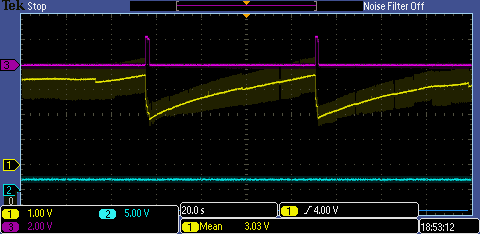
\includegraphics[width=0.75\textwidth]{4Resultate/imag/pic_3.PNG}
    \caption{Senden von Paketen bei 9 - 10 km/h; rot: V\_SUP, gelb: V\_STS}
    \label{paket_100kmh}
\end{figure}

Bei 16 km/h verkürzt sich die Ladezeit auf 10 s (siehe Abbildung \ref{paket_16kmh}). Die Fahrerin bzw. der Fahrer erhält alle 20 s einen aktuellen Wert. Trügerisch in diesem Bild ist, dass LTS bereits geladen ist. Dies entsteht nicht durch 16 km/h, sondern entstand durch vorangehende Messungen mit höheren Geschwindigkeiten. Auf die Ladezeit des STS hat dies keine Auswirkung.

\begin{figure}[ht]
   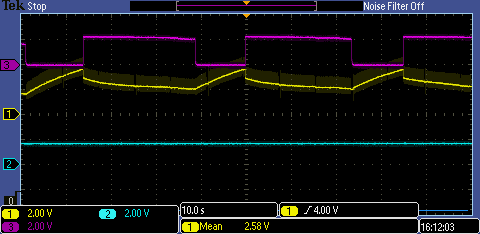
\includegraphics[width=0.75\textwidth]{4Resultate/imag/pic2.PNG}
    \caption{Senden von Paketen bei 16 km/h; rot: V\_SUP, gelb: V\_STS, blau: V\_LTS}
    \label{paket_16kmh}
\end{figure}

Bei 40 km/h werden rund 15 BLE-Pakete mitgesendet, bis V\_STS (gelb) unter den Schwellwert fällt und V\_SUP (viollet) abstellt (Abbildung \ref{paket_40kmh}). Danach dauert es nicht ganz 2 Sekunden, bis wieder nonstop gesendet wird und zwar für für die nächsten 2.5 Sekunden. Bei 40 km/h werden alle Sensoren im Ringbufferprinzip ausgelesen: beim ersten Paket wird der Druck aktualisiert, danach die Temperatur, dann die Luftfeuchtigkeit. LTS lädt sich bei dieser Geschwindigkeit nicht, da V\_STS nur bis zum Schwellwert zur Speisung von V\_SUP gelangt und nie höher steigt.

\begin{figure}[ht]
   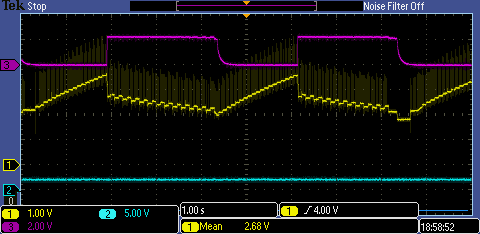
\includegraphics[width=0.75\textwidth]{4Resultate/imag/pic4.PNG}
    \caption{Senden von vielen Paketen bei 40 km/h}
    \label{paket_40kmh}
\end{figure}


\subsection{Laden und Entladen des LTS}
\label{res_entladen}

Das zweite Ziel, dass die vom LTS gespeicherte Energie für das Versenden der BLE-Pakete genutzt wird, wird in diesem Unterabschnitt erklärt. Die Bedingung nach Konzept des EM8500, dass VSTS den Schwellwert von v\_appl\_max\_\_lo von 3.7 V erreicht (siehe Schwellwerte graphisch dargestellt in Abbildung \ref{lts_ein}). In der Konfiguration wurde dieser Schwellwert so nah wie möglich an der Schwelle zu 3.6 V gewählt. Die Idee ist, sobald einmal V\_SUP konstant gespiesen ist, beginnt LTS unmittelbar mit dem Laden. Die Abbildung \ref{lts_ein} zeigt die finalen Einstellungen, zum  möglichst raschen Laden von LTS.

\begin{figure}[ht]
   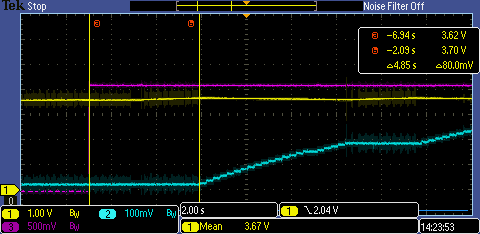
\includegraphics[width=0.75\textwidth]{4Resultate/imag/LTS_Ladeschwelle.PNG}
    \caption{Einschalten von LTS nach Schwellwert von 3.7 V}
    \label{lts_ein}
\end{figure}

Dies ist erst möglich, wenn VSUP konstant gespiesen wird. Denn nur in diesem Fall kann VSTS über den Schwellwert zur Speisung der Applikation von 3.6 V steigen und die Schwelle für die Speisung des LTS bei 3.7 V aktivieren. Dies gelingt ohne Sleep-Optimierung ab einer Geschwindigkeit von 50 km/h. Die Abbildung \ref{vsup_konstant} zeigt dies bei 60 km/h. LTS hat sich bereits auf die Höhe des STS von 3 V geladen. Ab einer Höhe von 3.6 V laden und entladen sich die beiden Kondensatoren parallel. Sie befinden sich im Connected Mode (siehe Datenblatt,  S. 6). Der Connected Mode ist in Abbildung \ref{connected_mode} dokumentiert.

\begin{figure}[ht]
   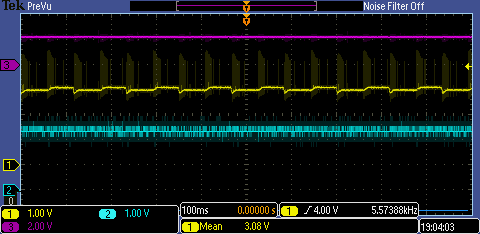
\includegraphics[width=0.75\textwidth]{4Resultate/imag/pic_5.PNG}
    \caption{VSUP wird konstant gespiesen. LTS lädt sich.}
    \label{vsup_konstant}
\end{figure}

\begin{figure}[ht]
   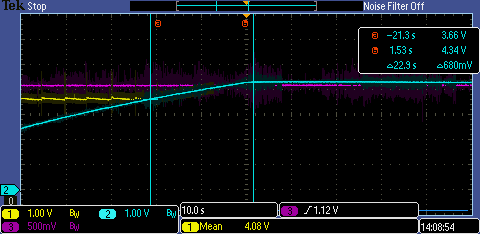
\includegraphics[width=0.75\textwidth]{4Resultate/imag/STS_LTS_connect.PNG}
    \caption{Connedted Mode der zwei Speicher}
    \label{connected_mode}
\end{figure}

Die letzte Abbildung (\ref{parallel_entladen}) zum Verhalten des LTS zeigt, wie STS und LTS im Parallelbetrieb sich entladen, V\_SUP sich halten kann und beide sich wieder parallel laden. 

\begin{figure}[ht]
   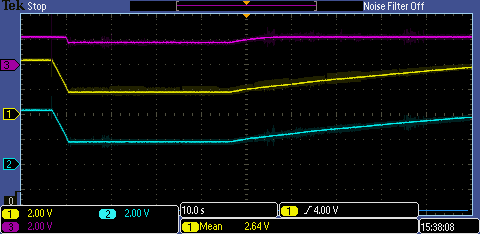
\includegraphics[width=0.75\textwidth]{4Resultate/imag/pic1.PNG}
    \caption{Paralleles Entladen und Wiederaufladen der Kondensatoren}
    \label{parallel_entladen}
\end{figure}

Diese Bilder belegen, dass das Laden und Entladen von LTS gut funktioniert. Das Problem liegt darin, dass bei der (noch nicht sleep-optimierten) TI-SensorTag Version V4 die Sensoren zu viel Energie verbrauchen und V\_SUP abfällt. Dadurch kommt es nicht zum Laden des LTS. Erst bei 50 km/h ist das Verhalten exemplarisch demonstrierbar. Es ist davon auszugehen, dass bei einer sleep-optimierten TI-SensorTag-Version das Laden und Entladen von LTS bereits bei tiefen Geschwindigkeiten funktioniert.

\subsection{Verwendete Werte}
\label{werte}

Die oben aufgeführten Messwerte sind mit der Software-Version V4 für das TI-Sensortag und den nachfolgenden, genannten Werten umgesetzt. Die Herleitung der Werte steht in den Unterkapiteln Energiekalkulation \ref{v_e_kalkulation} und Schwellwerte 3.4.3. Zwei Änderungen der Schwellwerte werden aufgrund letzter Messungen vorgenommen. Die Applikationsspeisung (V\_SUP) wird um 0.1 V auf 2.1 V erhöht. Der Grund ist, dass die Speisung bei 2 V, dem Minimum für das TI-SensorTag nicht 100\thinspace\% funktioniert. Das TI-SensorTag stellte teils selbständig ab, da angeblich zu wenig Spannung am Eingang anliegt. Um die gleiche Spannungsdifferenz von $\Delta$ 0.8 V zwischen STS\_HIGH und STS\_LOW zu haben, wird parallel dazu auch  v\_bat\_min\_hi\_dis erhöht. Der neue Wert ist nun 3.0 V, um sicher genügend Energie zur Verfügung zu stellen.

%Gleichung berechung totalenergie = 189 u J  \label{eq:e-high-e-low}
%Gleichung Berechnung CSTS ) 100 uJ         \label{eq:e_sts}
%Gleichung: STS_HIGH = 3 V    \ref{eq:bat_min_low_schwellwert}              

\begin{tabbing}
STS = 100 $\mu$F \hspace{1cm} \= (siehe Gleichung \ref{eq:e_sts})\\
LTS = 3300 $\mu$F             \> (Wert von Vorgängermodell behalten)
\end{tabbing}

\begin{minipage}{\textwidth}
\captionof{table}{Schwellwerte Energy Management Bicycle Computer}
    \begin{tabbing}
        Register \hspace{2cm} \quad\= Spannungswert \\[0.8ex]
        v\_bat\_max\_hi       \> 3.8 V \\
        v\_bat\_max\_lo       \> 3.7 V \\
        v\_bat\_min\_hi\_dis  \> 3.0 V  (STS\_HIGH)\\
        v\_bat\_min\_hi\_con  \> 2.2 V \\
        v\_bat\_min\_lo       \> 2.1 V (STS\_LOW)\\
        v\_appl\_max\_hi      \> 3.8 V \\
        v\_appl\_max\_lo      \> 3.7 V \\   
        mpp-ration            \> 60\thinspace\%
    \end{tabbing}
\end{minipage}  



\section{Energiebilanz}
\label{energiBilanz}
Das vorangehende Unterkapitel Energy Managment zeigt die erzielten Resultate. Dieses Kapitel liefert die Deutung dazu. Dazu wird aus der Tabelle \ref{tab_zsm} im Unterkapitel Energiemessungen der Energieverbrauch nach Aufgaben übernommen und in Zusammenhang mit der gelieferten Energie am EM8500-Ausgang gestellt. Die Energiedaten für den Ausgang des EM8500 stammen aus den Messungen \ref{em_enerige_ausgang}, die in der Tabelle \ref{tab:em_out_zsm} zusammengefasst sind.

\subsection{Energiebilanz Bicycle Computer}

Da der Sockelbeitrag an Energie für ein erstes Aufladen der Kondensatoren des TI-SensorTags wie auch des Energiespeichers STS gross ist (siehe  Abbildung \ref{r_bild_e_zusammenfassung}), wird zwischen den Startbedingungen, in denen dieses einmalige Aufladen erfolgt und der Nutzung des Bicycle Computers nach einer Minute Fahrzeit unterschieden.


\subsubsection{Energiebilanz beim Beginn der Fahrradnutzung}

Die Abbildung \ref{r_bild_e_zusammenfassung} zeigt in horizontalen Balken den Pegel des Energieverbrauchs des TI-SensorTags dar. Unterschieden wird zwischen dem einmaligen Laden (violett), der Initalisierung (rot) und dem Lesen und Senden der Daten (grau). Total ergibt sich ein Energiebedarf von 203 $\mu$J wie dies in der Gleichung \ref{eq:e-high-e-low} berechnet wird. Die eingetragene grüne Kurve stellt die zur Verfügung stehende Energie am EM8500-Chipausgang dar. Die Datenquellen und die exakten Werte stehen in der Tabelle \ref{everbrauch_aufgaben} unterhalb der Abbildung \ref{r_bild_e_zusammenfassung}.

\begin{figure}[ht]
     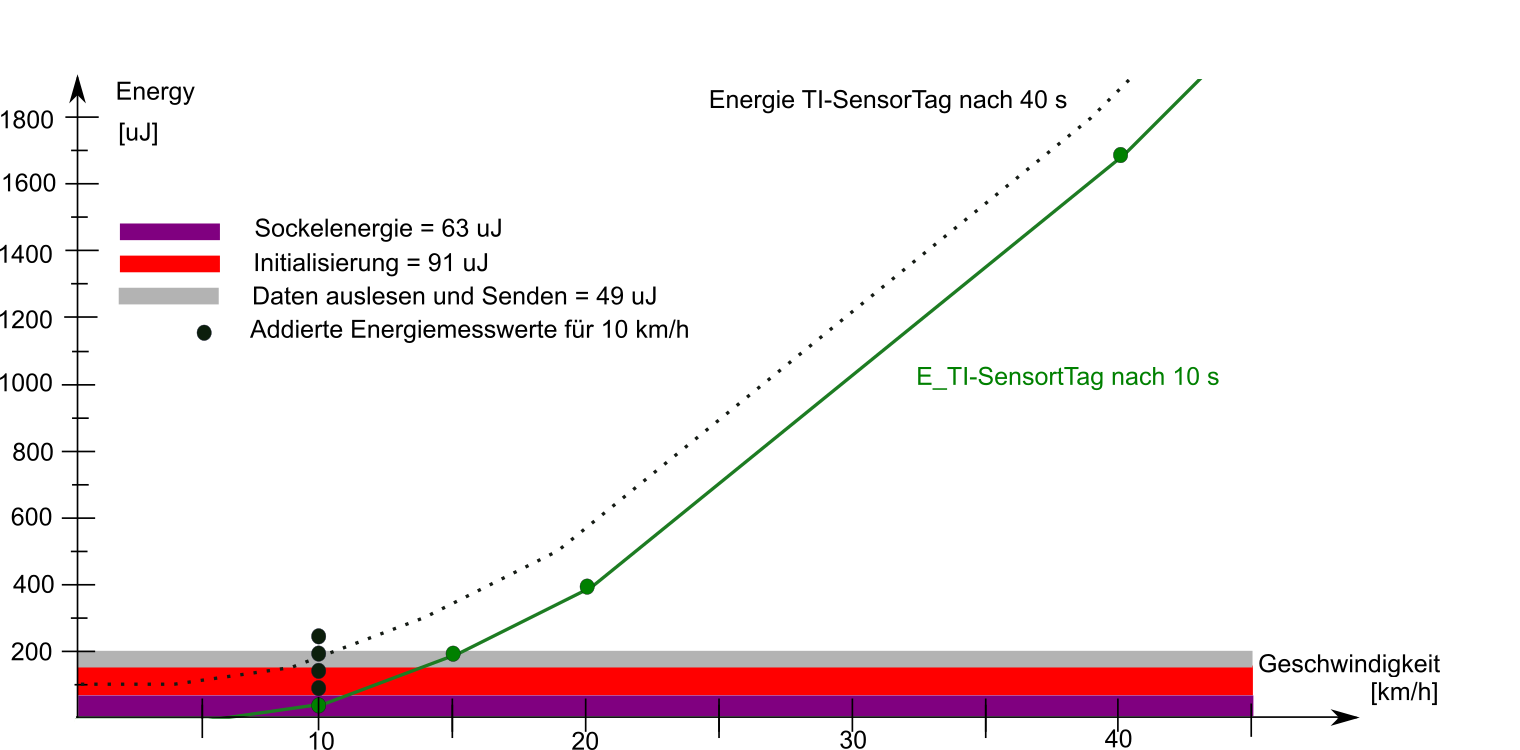
\includegraphics[width=1\textwidth]{4Resultate/imag/EnergyVerbrauchZusammenfassung.png}
     \caption{Energieverbrauch gem\"{a}ss Verarbeitungsaufwand für CPU}
     \label{r_bild_e_zusammenfassung}
\end{figure}

\begin{minipage}{\textwidth}
\captionof{table}{Energieverbrauch nach Aufgaben}\label{everbrauch_aufgaben}
    \begin{tabbing}
    Aufgabe \hspace{6 cm} \quad\=  Farbe \quad\= Energieverbrauch \hspace{1cm} \quad\= Quelle \\[0.8ex]
    Laden C TI-SensorTag  \> violett      \> 63 $\mu$J    \> Tabelle 3.8\\
    Initialisierung + Refresh-Zyklen \> rot \> 77 $\mu$J + 14 $\mu$J = 91 $\mu$J \> Tabelle 3.8\\
    Start Sensor + Geschwindigkeit, Daten BLE\> grau \> 6 $\mu$J + 43 $\mu$J = 49 $\mu$J    \> Tabelle 3.8\\
    Gesamtverbrauch TI-SensorTag     \>     \> 203 $\mu$J    \> Gleichung \ref{eq:e-high-e-low}\\
    \end{tabbing}
\end{minipage}



Die Abbildung \ref{r_bild_e_zusammenfassung} zeigt, dass bei der TI-Sensortag-Applikation V4 (siehe Messprotokoll \ref{messung_energie_sensortag}) innerhalb von 10 s nicht genug Energie für den Beginn der Fahrradnutzung bereit steht. Wartet die Fahrerin bzw. der Fahrer jedoch länger so addiert sich die gesammelte Energie (siehe Tabelle \ref{tab_zeit_aufsummiert}). Bei einem minimalen Energieverbrauch von 203 $\mu$J, sollte bei einem Neubeginn der Nutzung des Fahrrad-Computers nach 40 s das erste Datenpaket gesendet werden. Die Wiederholungsrate, mit der neue Pakete bei aufgeladenem System gesendet werden, wird im nächsten Unterkapitel dokumentiert.

\begin{minipage}{\textwidth}
\captionof{table}{Gesammelter Energieverbrauch für 10 km/h}
\label{tab_zeit_aufsummiert}
    \begin{tabbing}
    Zeit  \quad\=  Energievorrat \quad\= Quelle\\[0.8ex]
    10 s  \> 54.4 $\mu$J   \>  Messung \textbf{xxxx} \\
    20 s  \> 108.8 $\mu$J  \> \\
    30 s  \> 163.2 $\mu$J  \> \\
    40 s  \> 217.6 $\mu$J  \> \\
    50 s  \> 272.0 $\mu$J  \> \\
    \end{tabbing}
\end{minipage}

\todo{Referenz einbauen}

\subsection{Energiebilanz nach 1 min Fahrzeit}

Fällt das Aufladen der TI-SensorTag-Kondensatoren weg, so sieht die Energiebilanz besser aus. Die Abbildung \ref{r_bild_e_zusammenfassung_ohneSockel} zeigt, dass bei einer Geschwindigkeit von 10 km/h nach 30 s genügend Energie zum Senden eines Paketes mit Sensordaten zur Verfügung steht. Zudem zeigt sich, dass mit zunehmender Geschwindigkeit kein Energieproblem mehr besteht. 


\begin{figure}[ht]
     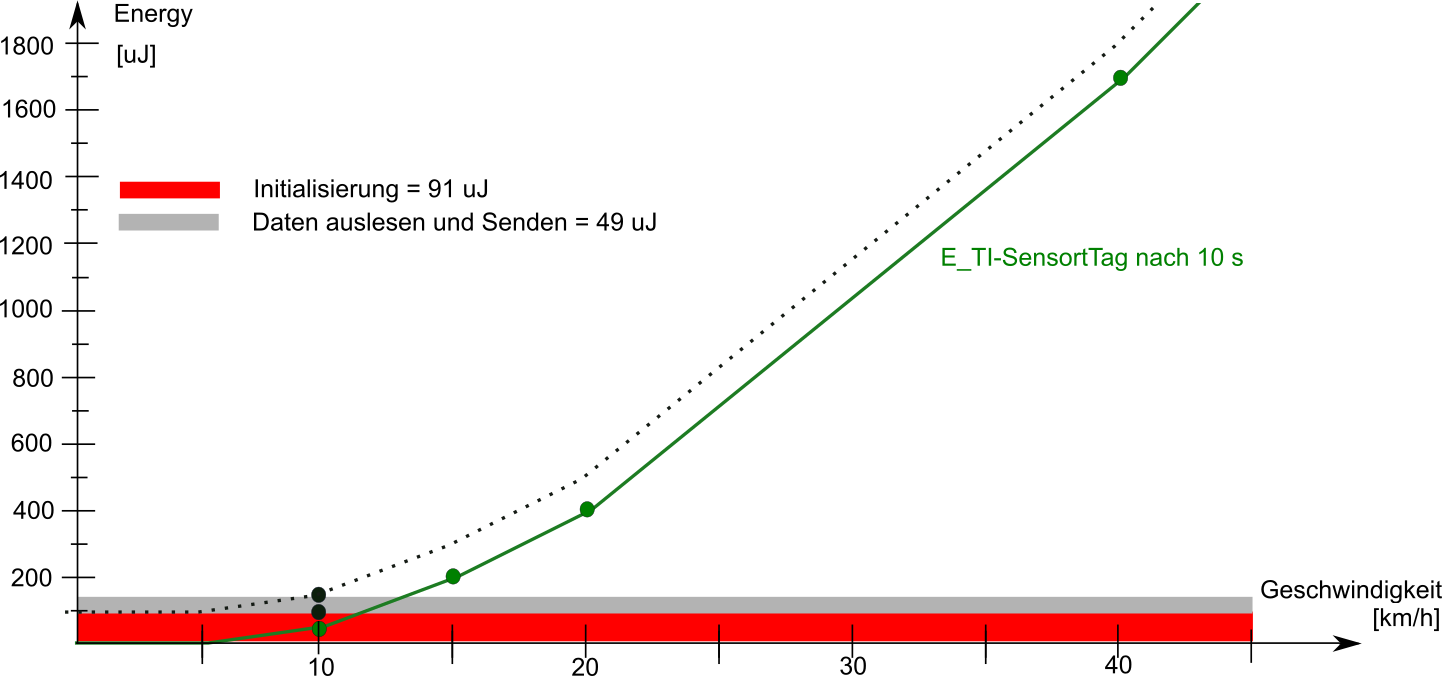
\includegraphics[width=1\textwidth]{4Resultate/imag/EnergyVerbrauchZusammenfassung_ohneSockel.png}
     \caption{Energieverbrauch gem\"{a}ss Verarbeitungsaufwand für CPU}
     \label{r_bild_e_zusammenfassung_ohneSockel}
\end{figure}

Die zur Verfügung stehende Energie ändert sich mit zunehmender Geschwindigkeit schnell.

% Startet man den Bicycle Computer neu, genügen braucht es 20 km/h, um nach 10 s ein Geschwindigkeitspaket zu erhalten. 
Zusammenfassend lassen sich über den Protoypen eines Fahrrad-Computers sagen:

\begin{minipage}{\textwidth}
\captionof{table}{Resultate Bicycle Computer}
    \begin{enumerate}
    \item Das Übermitteln der Geschwindigkeit und Sensordaten ist ab 10 km/h möglich
    \item Das Übermitteln erster Daten braucht bei 10 km/h rund 1.5 Minuten.
    \item Bei einer Geschwindigkeit von 20 km/h werden die Daten alle 20 s aktulisiert
    \item Bei einer Geschwindigkeit von 40 km/h werden die Daten alle 2 s aktulisiert
    \end{enumerate}
\end{minipage}


%Der Grund für die Schwierigkeit bei tiefer Geschwindigkeit liegt am hohen Sockelbetrag zum Starten des Systems. Der Short Time Storage muss zuerst auf die Höhe des Schwellwerts zur Speisung der Applikatin geladen werden. Dies bedeutet einen einmaligen Energieaufwand von 220 $\mu$J. Die Kondensatoren des TI-SensorTags müssen zu Beginn ebenfalls geladen werden. Dies sind weitere 63.2 $\mu$J. Zudem braucht die Initialisierung und das Refreshen zusammen in den ersten 10 s 90 $\mu$J. Zusammen ergibt dies einen Grundenergieverbrauch ab Start von 373.3 $\mu$J. Dies ist bei einer Geschwindikeit von 10 km/h erst nach xxx s möglich.
%
%\todo{Zeit bei 10km/h eintragen. Abschlusssatz besser}
%


\section{Ergebnisse BLE-Applikation}

Der Aufbau des TI-SensorTags zusammen mit dem selbst entwickelten Board wird ``Sensor'' genannt. Dies, weil aus der Sicht einer Benutzerin oder eines Benutzers keine detaillierte Hardware besteht, sondern ``ein Sensor''. Die Vereinfachung dient der Benutzerfreundlichkeit. Die Android-Applikation ist bewusst einfach aufgebaut, um die Benutzerin bzw. den Benutzer nicht zu verwirren. 

Der animierte Tachometer stellt die aktuelle Geschwindigkeit schnell und übersichtlich dar. Weitergehende Funktionen sind durch prägnante Namen selbsterklärend und der User sollte keine Mühe haben, die App ohne Lesen einer Anleitung zu verstehen.

\subsection{Applikationsstruktur}

Beim Öffnen der Applikation wird geprüft, ob Bluetooth aktiviert ist (siehe Abbildung \ref{permission}). Sollte Bluetooth nicht aktiviert sein, wird der User gefragt, ob Bluetooth aktiviert werden darf. Sollte der User die Aktivierung ablehnen schliesst sich die Applikation sofort.

\begin{figure}[ht]
 \begin{minipage}[t]{0.5\textwidth}
    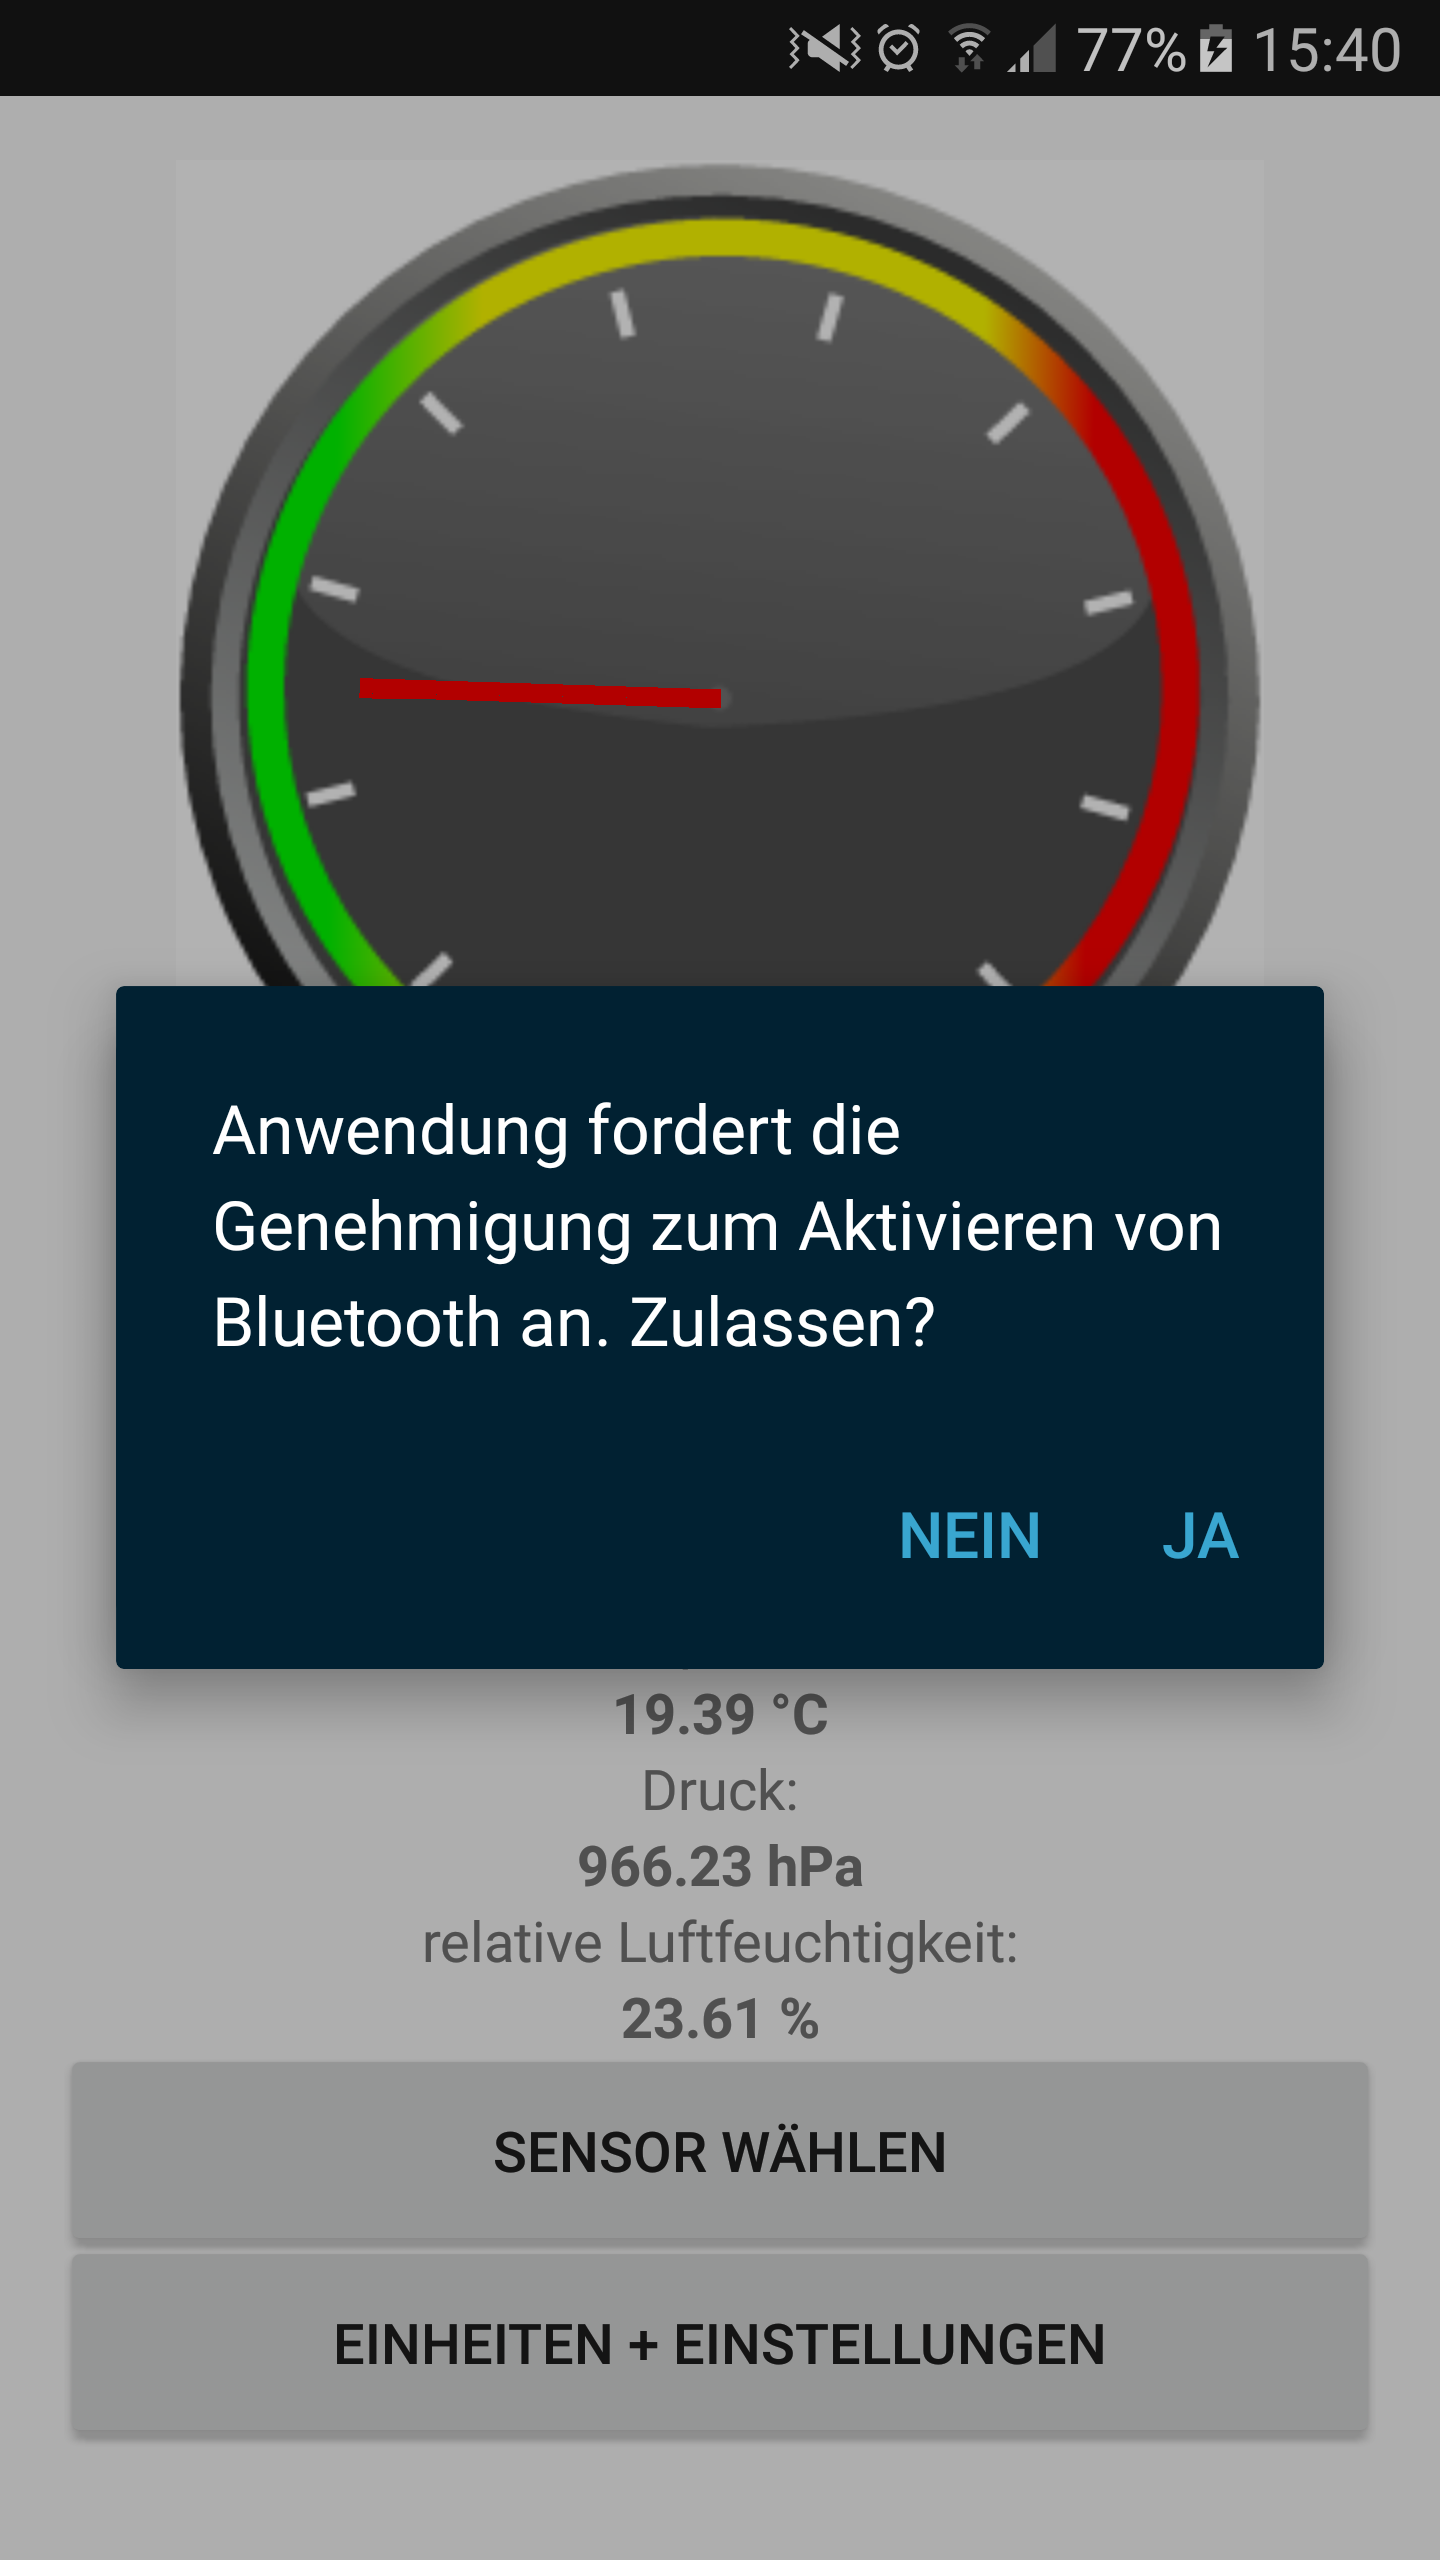
\includegraphics[width=0.9\textwidth]{4Resultate/imag/BLEBluetoothPermission.png} 
    \caption{Bluetooth Permission}
    \label{permission}
 \end{minipage}
 \begin{minipage}[t]{0.5\textwidth}
    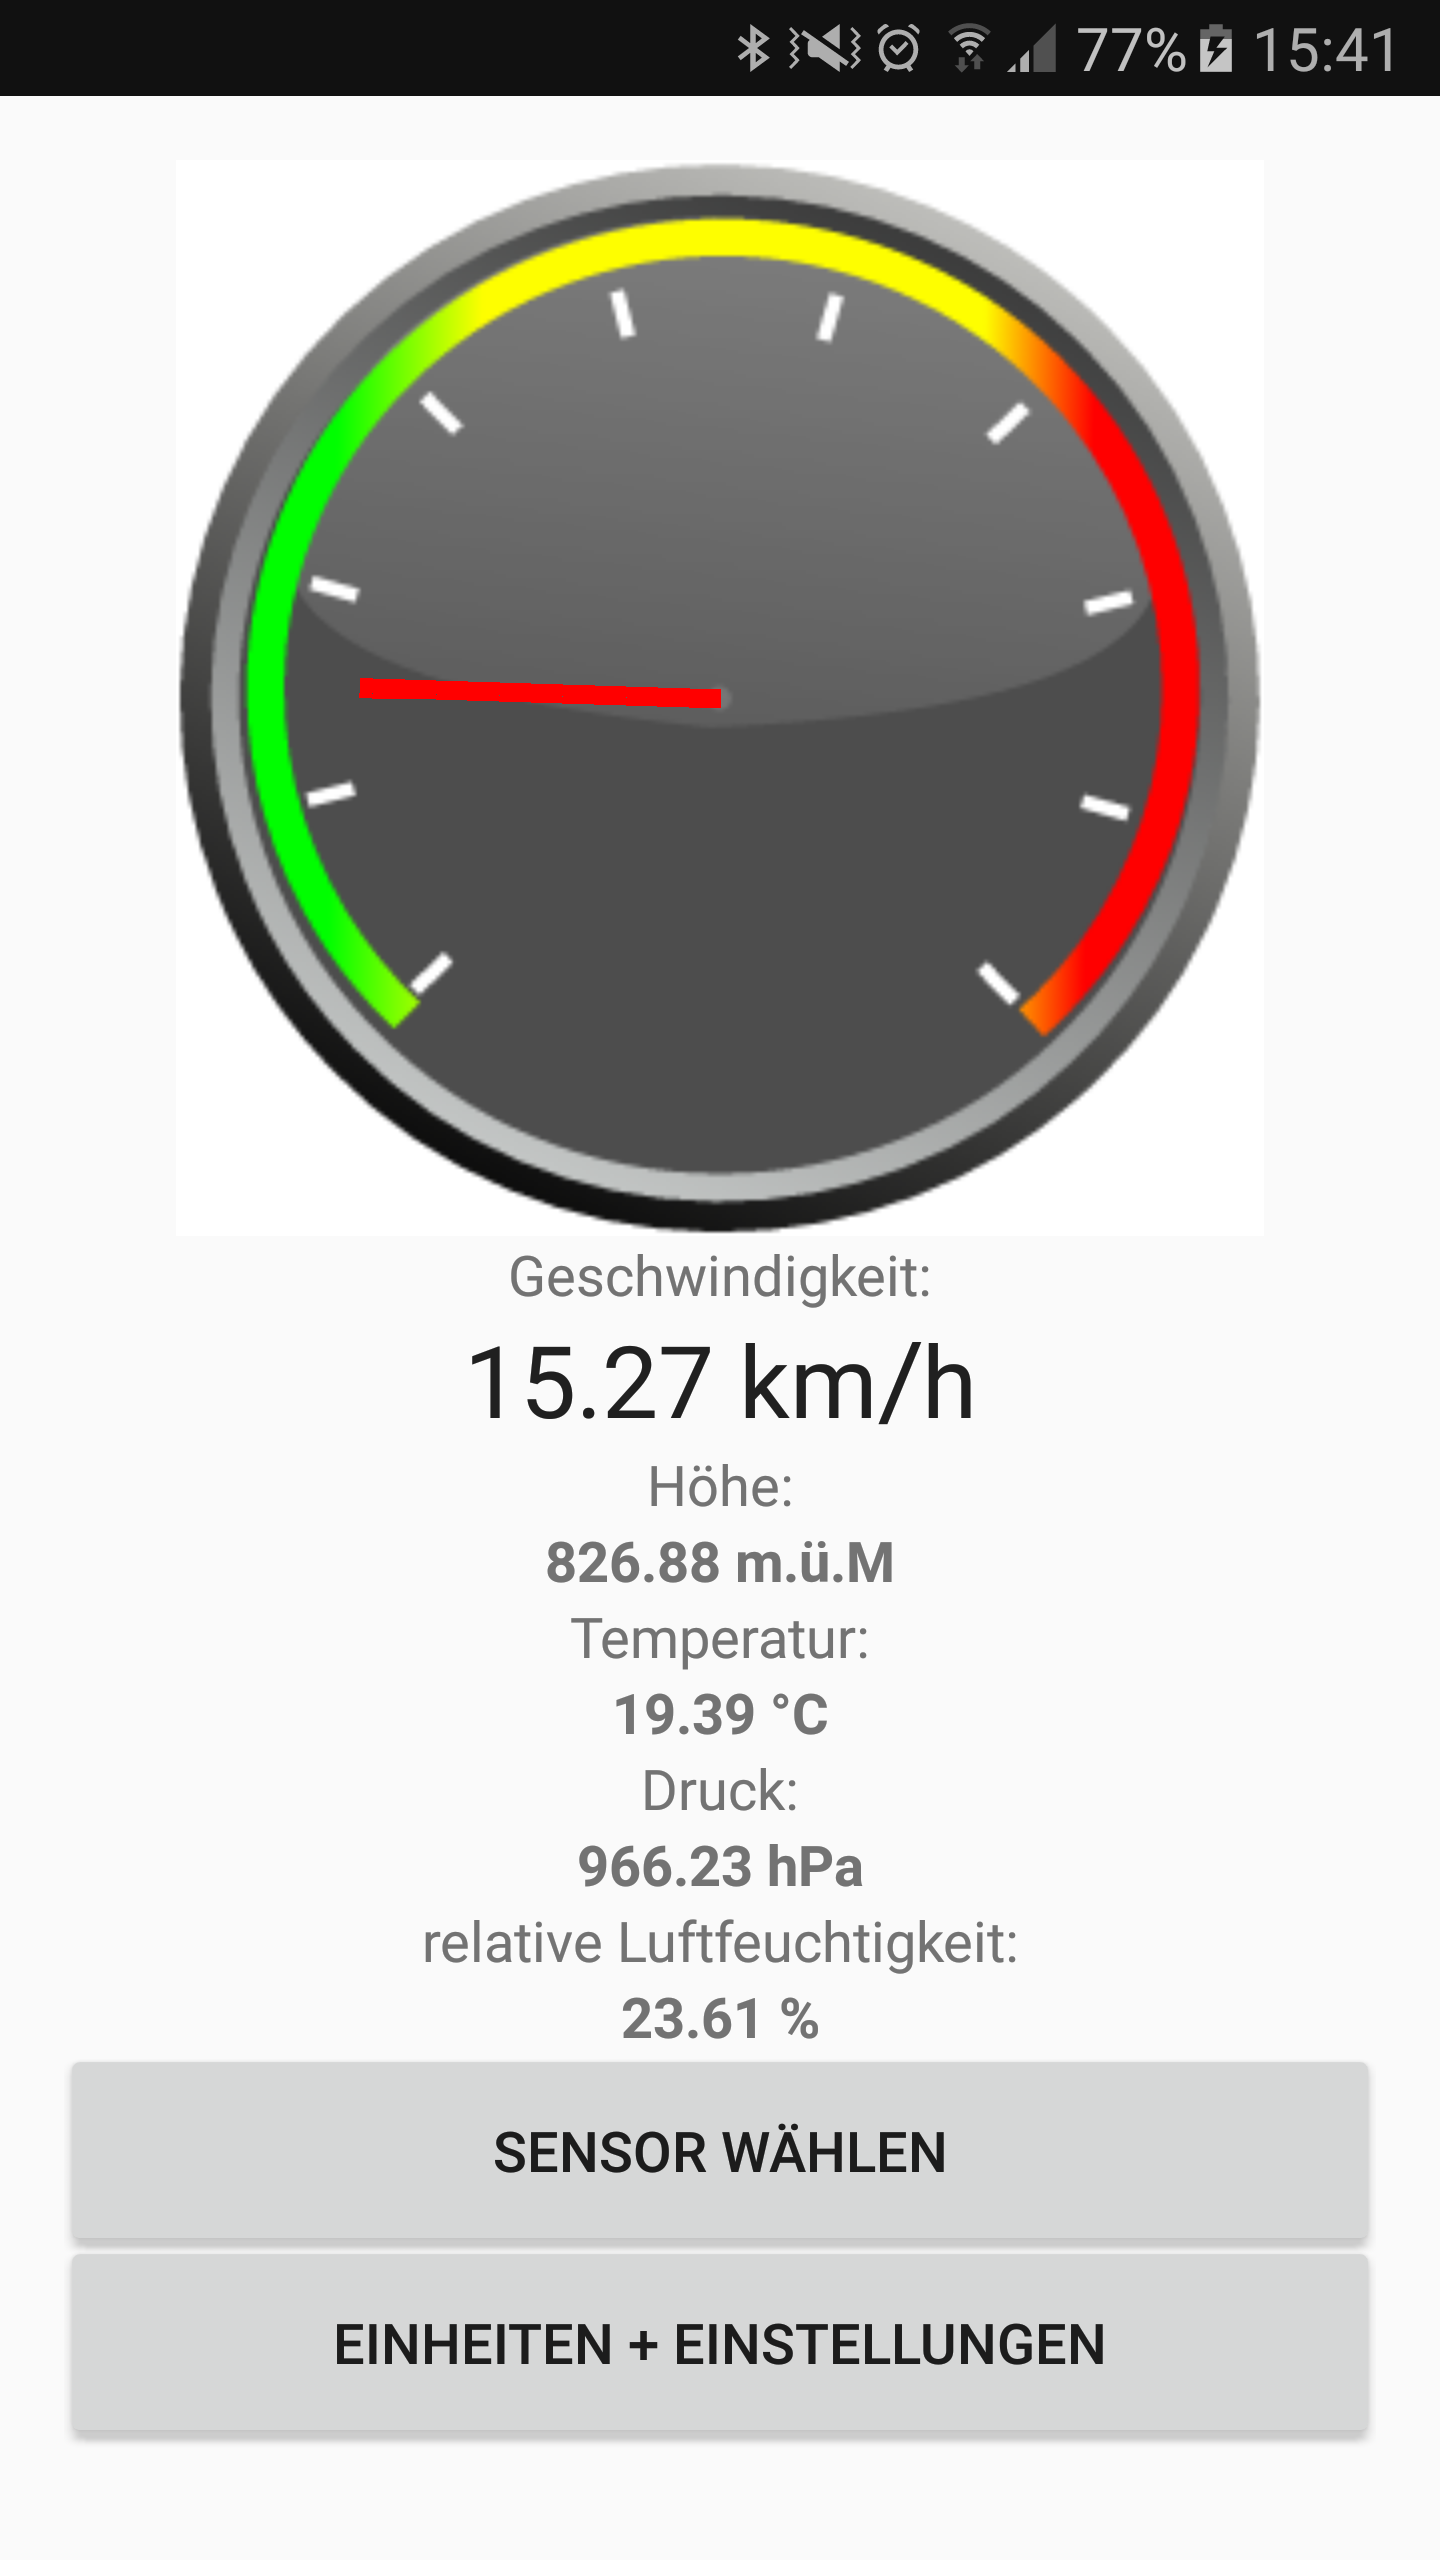
\includegraphics[width=0.9\textwidth]{4Resultate/imag/APPHomeScreen.png} 
    \caption{Startbildschirm der Applikation}
    \label{tacho}
 \end{minipage}
\end{figure}

Wird die Aktivierung der Bluetooth-Schnittstelle erlaubt, erscheint der Startbildschirm. Auf diesem befindet sich zentral der Tachometer (siehe Abbildung \ref{tacho}). Dieser zeigt Geschwindigkeiten von 0 – 90 km/h mit einer animierten Tachonadel an. Unterhalb des Tachometers werden die einzelnen Messwerte angezeigt und im untersten Teil des Startbildschirms befinden sich zwei Buttons, über die man Einstellungen vornehmen kann. Die Kontextmenus zu diesen Einstellungen werden in den nächsten zwei Abbildungen \ref{sensorauswahl} und \ref{einheiten} ersichtlich. 

Wählt man auf dem Startbildschirm ``Sensor wählen'', erscheint ein neuer Bildschirm. Auf diesem erscheinen nur die aktiven Bluetooth Geräte mit dem implementierten Prototypen-Filter. Der Bildschirm bildet die TI-SensorTag-Adresse ab. Der Verbund aus unserer neuen Leiterplatte und dem TI-SensorTag wird absichtlich als Sensor betittelt, da es sich für den User um ein Gerät handelt, welches Umgebungsdaten misst. Der User sieht das Gerät nicht in seinen Einzelteilen, sondern nimmt es als einen Sensor wahr. Es wird nicht der Sensor (Temperatursensor, Drucksensor, etc.) auf dem TI-SensorTag ausgewählt wird, sondern die Adresse des Bluetooth-Chips. Jedes TI-SensorTag hat eine eigene Adresse und bei mehreren Prototypen im Raum, kann das entsprechende Gerät ausgewählt werden, da die Adresse nicht sofort mit einem spezifischen TI-SensorTag in Verbindung gebracht werden kann.

\begin{figure}[ht]
 \begin{minipage}[t]{0.5\textwidth}
    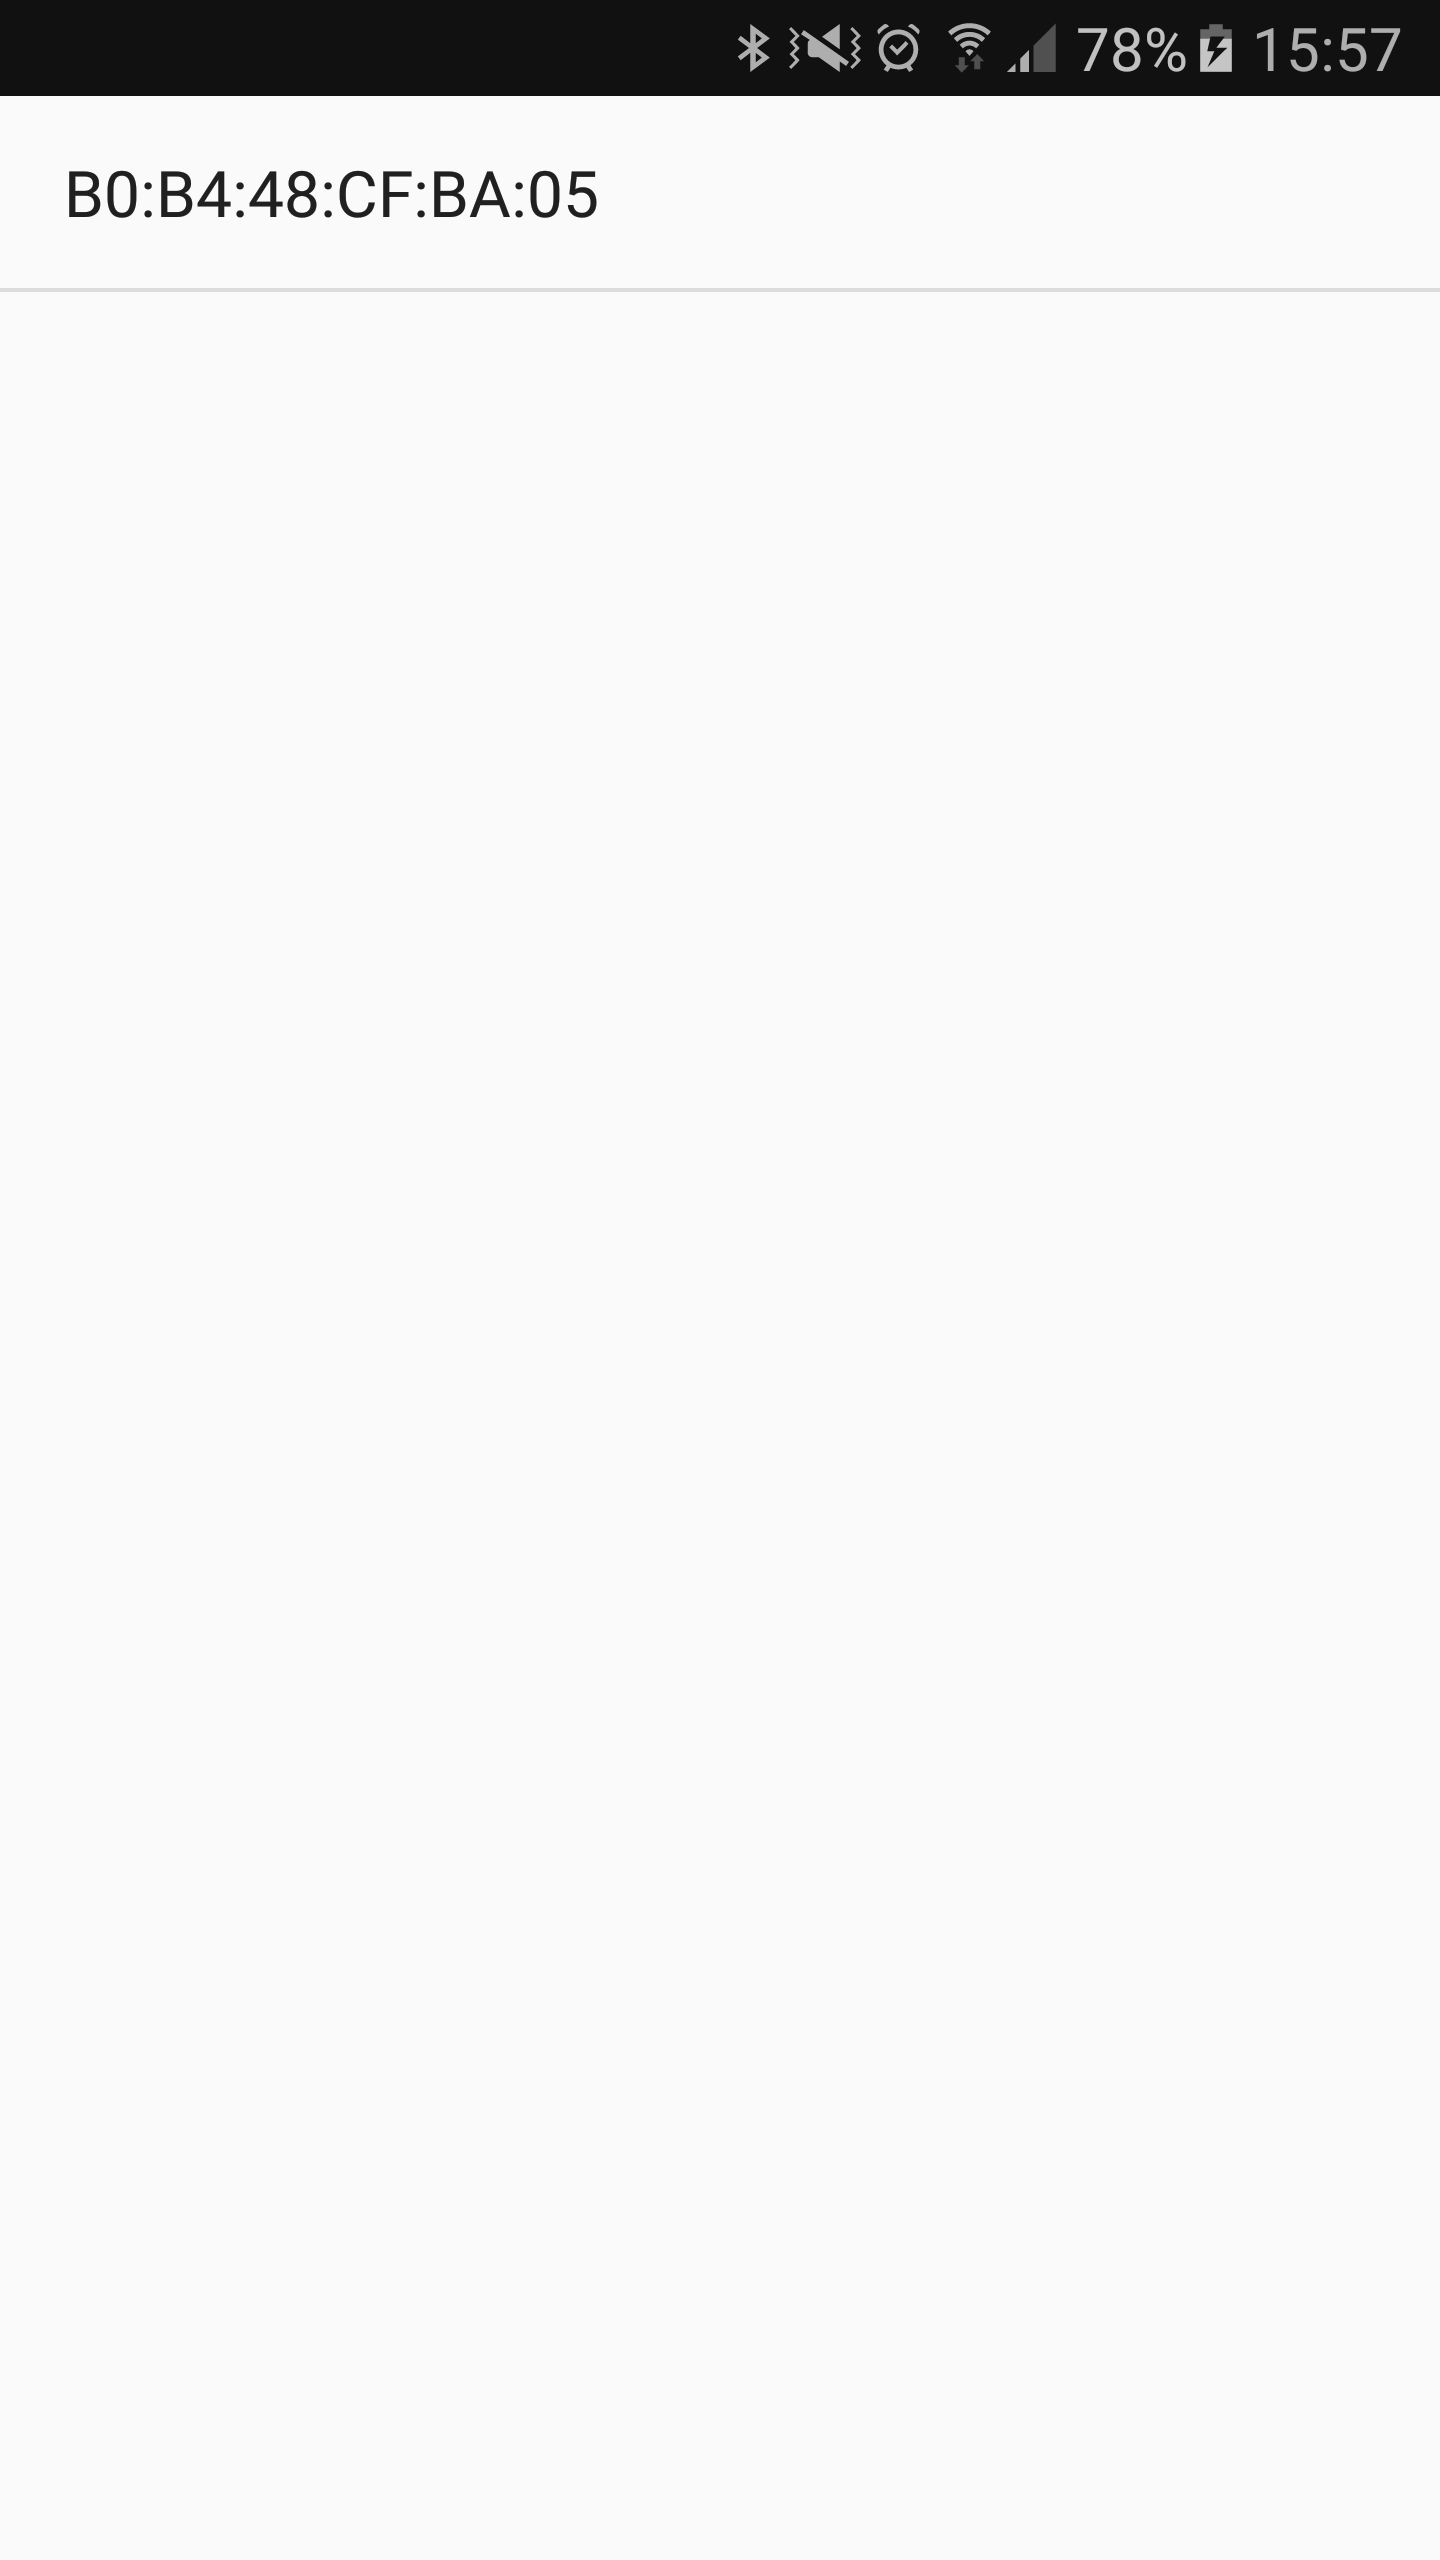
\includegraphics[width=0.9\textwidth]{4Resultate/imag/BLEAdresseAuswaehlen.png} 
    \caption{TI-SensorTagauswahl}
    \label{sensorauswahl}
 \end{minipage}
 \begin{minipage}[t]{0.5\textwidth}
    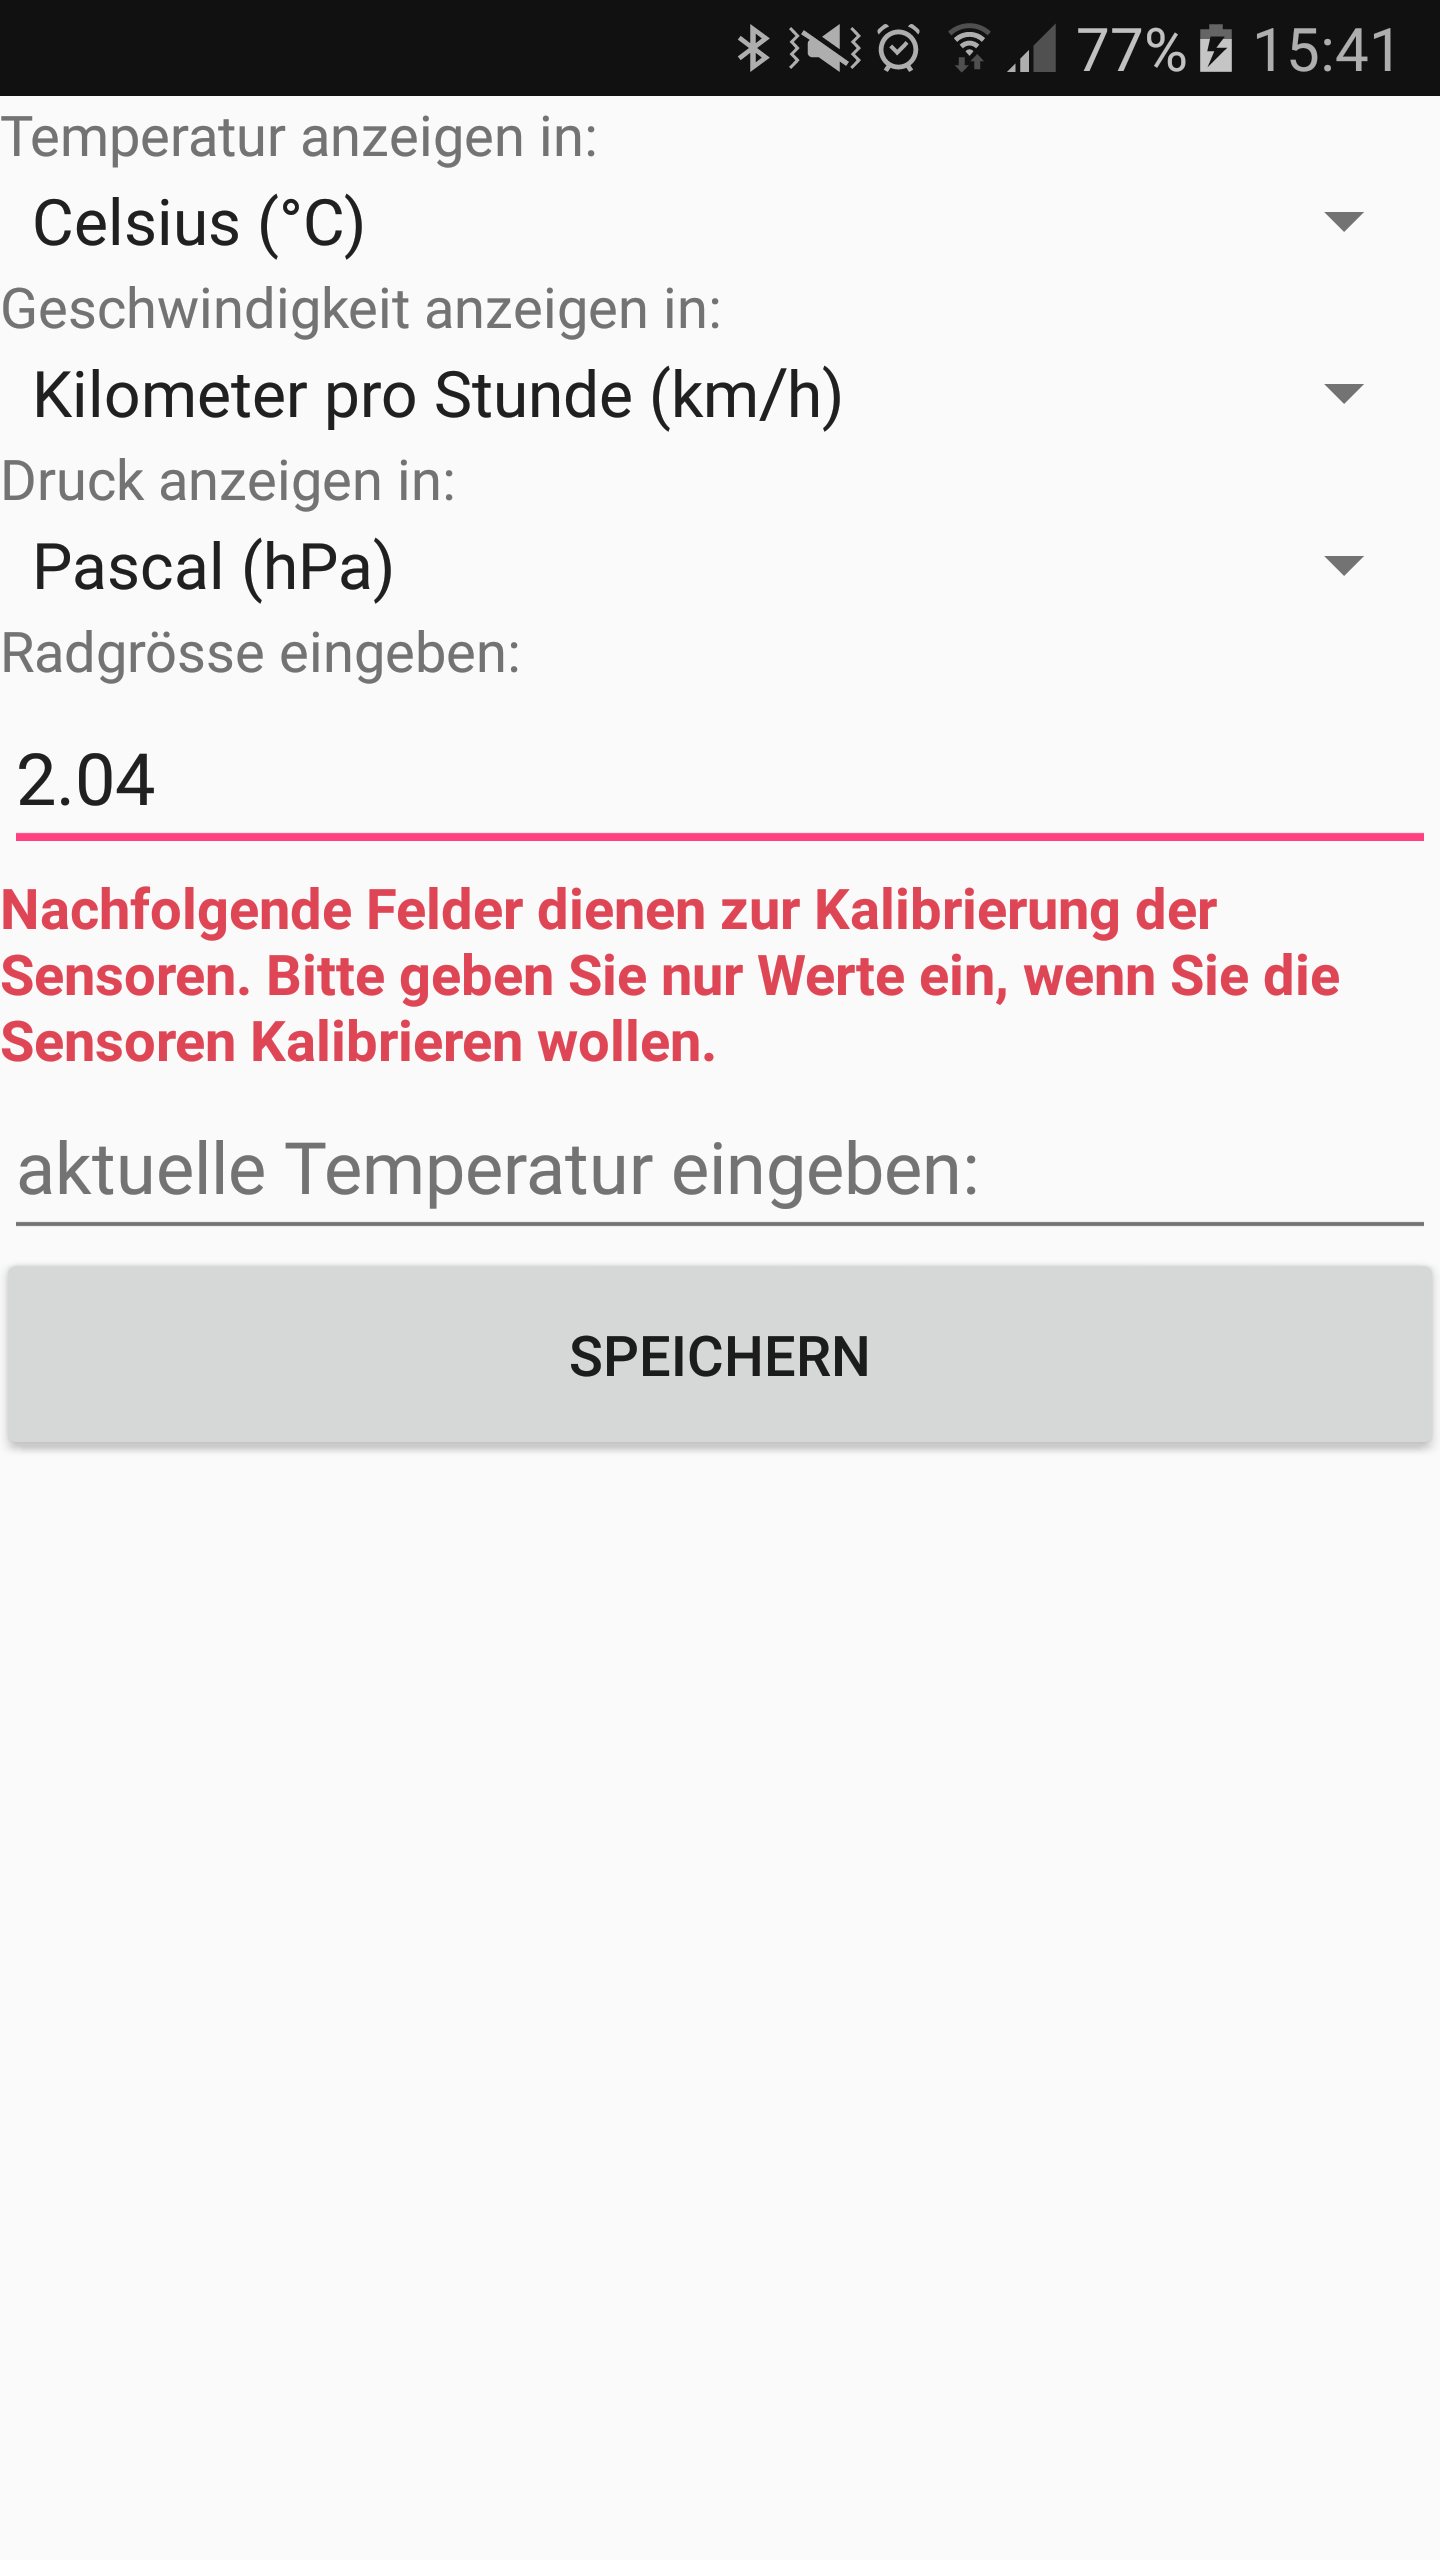
\includegraphics[width=0.9\textwidth]{4Resultate/imag/BLEEinheitenUndEinstellungenStart.png} 
    \caption{Einheiten und Einstellungen}
    \label{einheiten}
 \end{minipage}
\end{figure}

Auf dem Startbildschirm befindet sich auch ein Konfigurationsknopf. In das Untermenu gelangt man, indem man den Button ``Einheiten + Einstellungen'' auswählt.

Die Applikation stellt mehrere Konfigurationsmöglichkeiten zur Verfügung (siehe Abbildung \ref{einheiten}). Zu jedem Sensor gehört ein Drop Down-Element, in dem die Einheiten ausgewählt werden können. Neben der Einheitenauswahl verfügt die App über die Möglichkeit, den Radumfang anzupassen und die Temperatur zu kalibrieren. 

Die Zahl des Radumfangs kann über die Tastatur in das Feld eingegeben, es können nur Zahlen eingegeben werden. Dies wurde implementiert, um zu verhindern, dass die Eingabe von der Applikation nicht interpretiert werden kann.

Bei der Temperaturanzeige ist eine Kalibrierung eingebaut. Dies, weil alle drei Temperatursensoren auf dem TI-SensorTag einheitlich zu hohe Werte ausgeben. Der zu hohe Temperaturwert liegt am Aufbau des Prototypen. TI-SensorTag und Print liegen nahe aufeinander und es entsteht Wärme im Zwischenraum. Der Benutzer oder die Benutzerin kann den korrekten Wert im Kalibrationsfeld eingeben. Die nächste Temperatur, die empfangen wird, wird mit dem eingetragenen Wert verglichen und ein Offset wird eingestellt. Wird keine Kalibration eingetragen, wird die Temperatur nicht kalibriert und der Offset bleibt unverändert.

\begin{minipage}{\textwidth}
\captionof{table}{Auswählbare Einheiten}
    \begin{tabbing}
    Temperatur\hspace{.3cm} \quad\= Geschwindigkeit\hspace{2.7cm} \quad\= Druck \\[0.8ex]
    Celsius ($^{\circ}$C)    \> Kilometer pro Stunde (km/h)\> Pascal (haP)\\
    Fahrenheit ($^{\circ}$F) \> Miles per hour (mph)       \> Bar (bar)\\
    Kelvin (K)     \>                            \> Atmosph\"{a}re (atm)\\
                   \>                      \> Pound-Force per sqare inch (psi)\\
                   \>                      \> Millimeter Quecksilber (mmHG)\\
    \end{tabbing}
\end{minipage}
  
Die vorgenommenen Einstellungen werden über den Button ``Speichern'' gesichert. Danach werden die eingelesenen Sensordaten in den ausgewählten Einheiten dargestellt.

\subsection{Paketverlust}

TI-SensorTag sendet im Advertising Mode drei Pakete pro Sendevorgang. Gemessen wird der Paketverlust bei einer Geschwindigkeit von 20 km/h (siehe Tabelle \ref{BLEPaketverlust} und \cite{messung_BLE}). 

\begin{minipage}{\textwidth}
\captionof{table}{Paketverlust BLE-Applikation}\label{BLEPaketverlust}
    \begin{tabbing}
    Messperiode \quad\= Gesendete Pakete \quad\= Empfangene Pakete \quad\= Paketverlust\\[0.8ex]
    1 min  \> 38   \> 35 \> 7.9\thinspace\%  \\
    1 min  \> 37   \> 31 \> 16.2\thinspace\%  \\
    2 min  \> 75   \> 64 \> 14.7\thinspace\%  \\
    2 min  \> 77   \> 65 \> 15.6\thinspace\%  \\
    5 min  \> 193   \> 168 \> 13.0\thinspace\%  \\
    5 min  \> 190   \> 158 \> 16.8\thinspace\%  \\
    10 min  \> 345   \> 301 \> 12.8\thinspace\%  \\
    10 min  \> 349   \> 302 \> 13.5\thinspace\%
    \end{tabbing}
\end{minipage}

\subsection{Korrektheit der Daten}

Die Korrektheit der empfangenen Daten auf der Applikation wird mit einem visuellen Vergleich der Datenpakete im BLE-Sniffer von TI verglichen (siehe Abbildung \ref{sniffer}).  Die Daten im Sniffer entsprechen exakt den Daten, welche die Applikation empfängt. Der Inhalt der Daten wird somit unverfälscht übermittelt.

\begin{figure}[ht]
    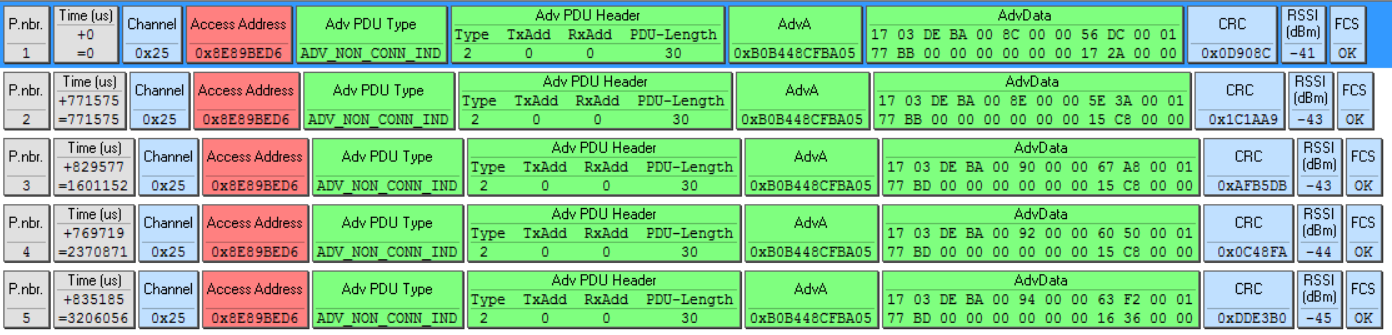
\includegraphics[width=1.0\textwidth]{4Resultate/imag/sniffer.png} 
    \caption{Empfangende Daten des Sniffers}
    \label{sniffer}
\end{figure}

\begin{figure}[ht]
    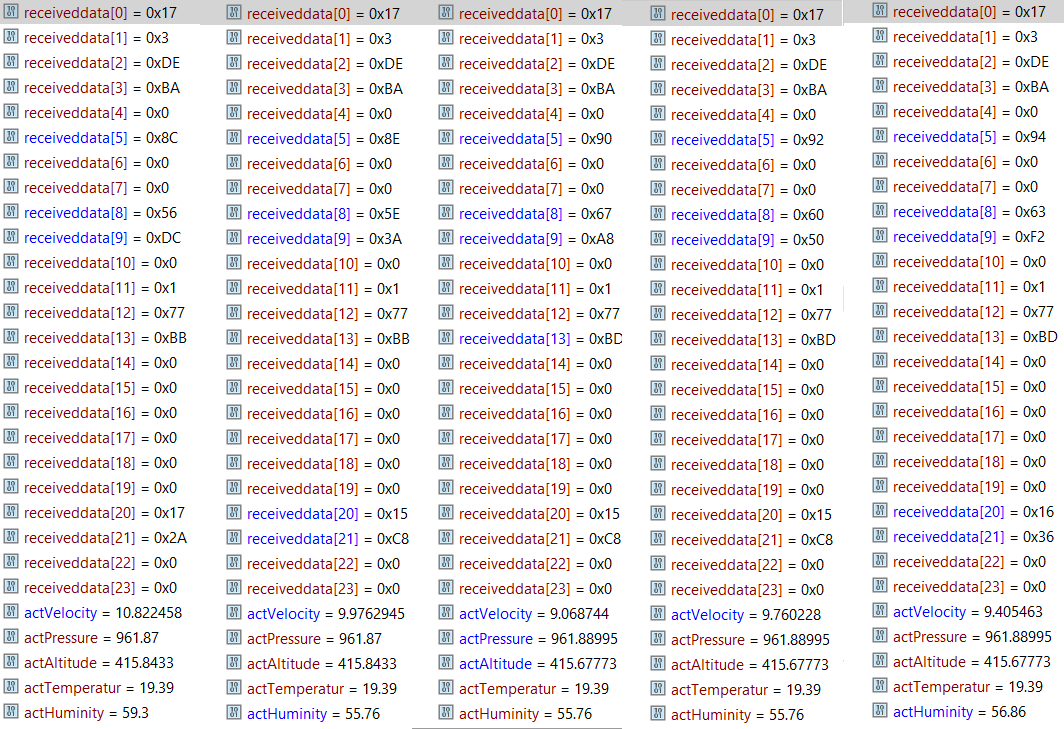
\includegraphics[width=1.0\textwidth]{4Resultate/imag/app_alle.png} 
    \caption{Empfangene Daten der Applikation}
    \label{applikation_daten}
\end{figure}


\todo{Video zeiger (auf CD)}
